\documentclass[12pt,a4paper]{paper}
\usepackage[utf8]{inputenc}
\usepackage[english]{babel}
\usepackage{amsmath}
\usepackage{enumitem}
\usepackage{arydshln}
\usepackage{amsfonts}
\usepackage{multirow}
\usepackage{multicol}
\usepackage{vwcol}
\usepackage{amssymb}
\usepackage{tikz}
\usepackage[left=1cm,right=1cm,top=1.5cm,bottom=2cm]{geometry}
\allowdisplaybreaks
\usepackage{Sweave}
\begin{document}
\title{GENE638 - Homework 4\\\small{Daniel Osorio - dcosorioh@tamu.edu\\Department of Veterinary Integrative Biosciences\\Texas A\&M University}}
\maketitle
\Sconcordance{concordance:HW4_DanielOsorio.tex:HW4_DanielOsorio.Rnw:%
1 14 1 1 0 89 1}

\begin{center}
\begin{tabular}{|c|c|c|c|}
\hline
COW&HERD&LACTATION&MILK FAT (lb)\\
\hline
1&1&1&600\\
\hline
1&1&2&680\\
\hline
2&1&1&500\\
\hline
3&2&1&800\\
\hline
3&2&2&895\\
\hline
4&2&1&775\\
\hline
5&2&1&600\\
\hline
5&2&2&715\\
\hline
\end{tabular}
\end{center}
Given $y_{ijk} = \mu + H_{i} + L_{j} + C_{k} + e_{ijk}$ where $\mu$, herd ($H_{i}$) and lactation $L_{j}$ are fixed effects; cows ($C_{k}$) and residuals ($e_{ijk}$) are random effects and $var\left[\begin{array}{c}\underline{c}\\\underline{e}\end{array}\right] = \left[\begin{array}{cc}A\sigma^{2}_{c}&0\\0&I\sigma^{2}_{e}\end{array}\right]$ so the MME are: $\left[\begin{array}{cc}X'X&X'Z\\Z'X&Z'Z+A^{-1}\lambda\end{array}\right]\times \left[\begin{array}{c}\underline{\hat{\beta}}\\\underline{\hat{u}}\end{array}\right]=\left[\begin{array}{c}X'\underline{y}\\Z'\underline{y}\end{array}\right]$ with $\lambda = \frac{\sigma^{2}_{e}}{\sigma^{2}_{c}}$.
\begin{enumerate}
\item In the above model, indicate what each subscript indexes.
\item What are the elements in $\underline{\hat{\beta}}$ and $\underline{\hat{u}}$
\end{enumerate}
New pedigree:
\begin{center}
\tikzset{every picture/.style={line width=0.75pt}} %set default line width to 0.75pt        
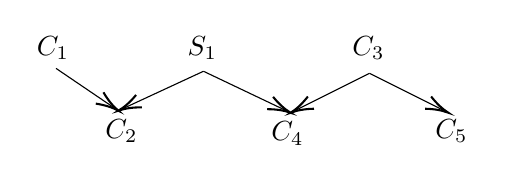
\begin{tikzpicture}[x=0.75pt,y=0.75pt,yscale=-1,xscale=1]
%uncomment if require: \path (0,300); %set diagram left start at 0, and has height of 300
%Straight Lines [id:da6398193474452144] 
\draw    (119.45,129.61) -- (147.85,148.88) ;
\draw [shift={(149.5,150)}, rotate = 214.16] [color={rgb, 255:red, 0; green, 0; blue, 0 }  ][line width=0.75]    (10.93,-3.29) .. controls (6.95,-1.4) and (3.31,-0.3) .. (0,0) .. controls (3.31,0.3) and (6.95,1.4) .. (10.93,3.29)   ;
%Straight Lines [id:da9832633356098646] 
\draw    (190.5,131) -- (151.31,149.16) ;
\draw [shift={(149.5,150)}, rotate = 335.14] [color={rgb, 255:red, 0; green, 0; blue, 0 }  ][line width=0.75]    (10.93,-3.29) .. controls (6.95,-1.4) and (3.31,-0.3) .. (0,0) .. controls (3.31,0.3) and (6.95,1.4) .. (10.93,3.29)   ;
%Straight Lines [id:da30378041653461985] 
\draw    (190.5,131) -- (230.69,150.14) ;
\draw [shift={(232.5,151)}, rotate = 205.46] [color={rgb, 255:red, 0; green, 0; blue, 0 }  ][line width=0.75]    (10.93,-3.29) .. controls (6.95,-1.4) and (3.31,-0.3) .. (0,0) .. controls (3.31,0.3) and (6.95,1.4) .. (10.93,3.29)   ;
%Straight Lines [id:da5090772911581323] 
\draw    (270.5,132) -- (234.29,150.11) ;
\draw [shift={(232.5,151)}, rotate = 333.43] [color={rgb, 255:red, 0; green, 0; blue, 0 }  ][line width=0.75]    (10.93,-3.29) .. controls (6.95,-1.4) and (3.31,-0.3) .. (0,0) .. controls (3.31,0.3) and (6.95,1.4) .. (10.93,3.29)   ;
%Straight Lines [id:da05497269582519504] 
\draw    (270.5,132) -- (306.71,150.11) ;
\draw [shift={(308.5,151)}, rotate = 206.57] [color={rgb, 255:red, 0; green, 0; blue, 0 }  ][line width=0.75]    (10.93,-3.29) .. controls (6.95,-1.4) and (3.31,-0.3) .. (0,0) .. controls (3.31,0.3) and (6.95,1.4) .. (10.93,3.29)   ;
% Text Node
\draw (118,120) node  [align=left] {$C_{1}$};
% Text Node
\draw (190,120) node  [align=left] {$S_{1}$};
% Text Node
\draw (270,120) node  [align=left] {$C_{3}$};
% Text Node
\draw (151,160) node  [align=left] {$C_{2}$};
% Text Node
\draw (231,161) node  [align=left] {$C_{4}$};
% Text Node
\draw (310,160) node  [align=left] {$C_{5}$};
\end{tikzpicture}
\end{center}
\begin{enumerate}[resume]
\item Calculate $A^{-1}$ using the Henderson's method for rapid inversion of $A$.
\item Write the observations in terms of the model $\underline{y} = X\underline{\beta}+Z\underline{u}+\underline{e}$
\item Construct MME with $\lambda = 1.5$
\item Show algebraically that $\lambda = \frac{1-h^{2}}{h^{2}}$
\item The row equation in the MME corresponding to $\hat{S}_{1}$ is:
\begin{equation*}
\begin{split}
0.75\hat{C_{1}} - 1.5\hat{C_{2}} + 0.75\hat{C_{3}} - 1.5\hat{C_{4}} + 3\hat{S_{1}} &= 0 \\
\hat{S_{1}} &= -0.25\hat{C_{1}} + 0.5\hat{C_{2}} - 0.25\hat{C_{3}} + 0.5\hat{C_{4}}\\
\hat{S_{1}} &= 0.5\left(\hat{C_{2}} - 0.5 \hat{C_{1}}\right) + 0.5\left(\hat{C_{4}} - 0.5 \hat{C_{3}}\right)
\end{split}
\end{equation*}
\begin{enumerate}
\item Look at the pedigree above (and this prediction equation) and describe in words how $\hat{S_{1}}$ is being predicted here.
\item Show that $\mu = 818.87$; $\hat{H}_{1}=-165.15$; $\hat{H}_{2} = 0$; $\hat{L}_{1}=-100.57$; $\hat{L}_{2}=0$; $\hat{C}_{1}=14.63$; $\hat{C}_{2}=-9.27$; $\hat{C}_{3}=31.57$; $\hat{C}_{4}=24.55$; $\hat{C}_{5}=-47.63$; and $\hat{S_{1}}$ (calculated as above) provides a solution to the system of equations.
\end{enumerate}
\item What do $\hat{H}_{1}$ and $\hat{L}_{1}$ estimate?
\item Show that $1'A^{-1}\hat{\underline{u}}=0$. What does this mean?
\item What are the predicted phenotypes $\hat{p} = \underline{y} - X\underline{\hat{\beta}}$
\item Find $\underline{\hat{e}}'\underline{\hat{e}}$ and compare results to those in Homework 3.
\item Do the predicted cow breeding values rank the same as they did in Homework 3 when all cows were treated as unrelated? Explain why or why not.
\end{enumerate}
\end{document}
